\chapter{Finite Difference}
There are several different variants of the  finite difference methods (FDMs), this is dependent on the stencil, the number of points being used to determine a single value. The use of a larger stencil yields a lower error, as can be seen in Figure \ref{fig:errorgraph} but also requires more computation time to generate a result.
%----------------------------------------------------------------------
\begin{figure}[H] 
 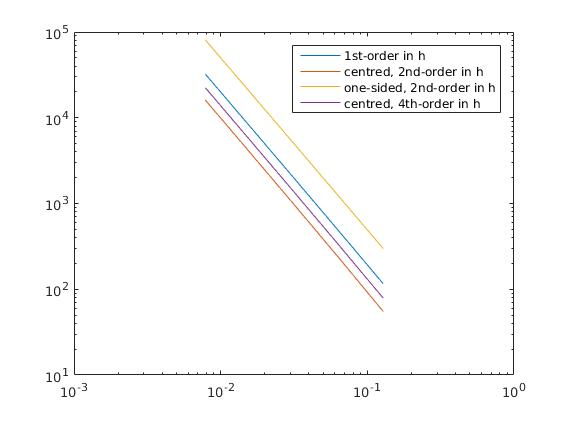
\includegraphics[width=\textwidth]{Images/Error.jpg}
 \caption{Comparison of Errors in FDM variants in log plot}
 \label{fig:errorgraph}
\end{figure}
%%%%%%%%%%%%%%%%%%%%%%%%%%%%%%%%%%%%%%%%%%%%%%%%%%%%%%%%%%%%%%%%%%%%%%%
\section{First Derivatives}
The FDM uses Taylor expansion to approximate the derivative of a function of finite points using the surrounding points such that $dv_i \approx \frac{df(x_i)}{dx}$.
\linebreak
\linebreak
The most basic of these is the first order FDM, given by Equation \ref{1ofdm}. It first order as the error in the function is relative to the spacing in the first order, $\epsilon \approx h$.
\begin{equation} \label{1ofdm}
  dv_i = \frac{v_{i+1} - v_i}{h}
\end{equation}
Equation \ref{1ofdm2c} has a centered stencil and uses two points giving it a lower error, $\epsilon \approx h^2$.
\begin{equation} \label{1ofdm2c}
  dv_i = \frac{v_{i+1} - v_{i-1}}{2h}
\end{equation}
Equation \ref{1ofdm2s} uses a three point stencil, but due to the fact that the stencil is one sided it is still of the second order, $\epsilon \approx h^2$.
\begin{equation} \label{1ofdm2s}
  dv_i = \frac{4v_{i+1} - v_{i+2} + 3v_i}{2h}
\end{equation}
Equation \ref{1ofdm4c} uses a four point, centered stencil to produce a fourth order approximation, $\epsilon \approx h^4$. As seen in Figure \ref{fig:errorgraph} this is the most accurate as it has the lowest error and the steepest gradient such that a smaller smaller spacing gives a much higher reduction in error compared to that of the other stencils.
\begin{equation} \label{1ofdm4c}
  dv_i = \frac{-v_{i+2} + 8v_{i+1} - 8v_{i-1} + v_{i-2}}{12h}
\end{equation}
%%%%%%%%%%%%%%%%%%%%%%%%%%%%%%%%%%%%%%%%%%%%%%%%%%%%%%%%%%%%%%%%%%%%%%%
\section{Second Derivatives}
Second derivatives are calculated in a similar manner to that of the first order and also have several variants depending on the stencil. It also uses the Taylor expansion to approximate the second derivative at a point such that $d^2v_i \approx \frac{df^2(x_i)}{dx^2}$.
\linebreak
\linebreak
The second ordered, centered stencil, seen in Equation \ref{2ofdm2c}, it is second order in h, which again means the error is relative to the spacing or $\epsilon \approx h^2$.
\begin{equation} \label{2ofdm2c}
  d^2v_i = \frac{v_{i+1} - 2v_i + v_{i-1}}{h^2}
\end{equation}
The fourth ordered, centered stencil, seen in Equation \ref{2ofdm4c} is more accurate than the second ordered, with $\epsilon \approx h^4$, but due to how complex it is compared to the second order, it is more expensive to calculate
\begin{equation} \label{2ofdm4c}
  d^2v_i = \frac{-v_{i+2} + 16v_{i+1} - 30v_i + 16v_{i-1} - v_{i-2}}{12h^2}
\end{equation}
%----------------------------------------------------------------------
\section{Ghost Points}
The problem with FDMs, especially with those of a higher order, is their reliance on points on either side of the point being calculated. This is impossible closer to the function boundaries as the points needed to calculate the derivatives at these points are not within the bounds of the function. This can be overcome by the introduction of ghost points, points outside of the bounds of the function, but which are still usable for the calculation of derivatives. These points are usually generated by treating the function as periodic over its domain and extending it as such, or by setting the points to zero. Both cases could lead to large errors in the approximation of the functions derivative if the points do not align with the actual points of the function at those positions.